% =====================================================================
%  Chapter 8 — Myopic Loss Aversion and the Evaluation Horizon
% =====================================================================

\chapter{Myopic Loss Aversion and the Evaluation Horizon}
\label{ch:myopic}

Chapter 7 established that the order of returns matters. This chapter
establishes something sharper and more uncomfortable: the \emph{order in
which the investor looks} changes the return the investor realises, and
does so by an amount comparable to the entire equity premium.

This is the most important behavioural result in long-horizon investing,
and it is also the one with the clearest practical implication in the
whole book. It is the reason the system is designed to be left alone.

\section{The mechanism}

Kahneman and Tversky's 1979 prospect theory gives the value function its
asymmetry: losses loom larger than equivalent gains. In the value
function, the slope of the utility curve in the domain of losses is
steeper than the slope in the domain of gains by a factor \(\lambda\), the
loss-aversion coefficient, which is estimated in the range 2 to 2.5.

Benartzi and Thaler combined this with a simple observation in 1995. An
investor who evaluates a portfolio once a year experiences one gain-or-loss
evaluation per year; an investor who evaluates weekly experiences
fifty-two. The reference point is reset at each evaluation, and the
asymmetry of the value function acts on each evaluation separately.

The consequence is that the investor's \emph{perceived} required return
depends on the evaluation frequency, and does so in a computable way. Let
the equity premium be \(\mu\) per year and the evaluation period be
\(T_E\) years. The investor perceives the risk of the evaluation period as
\(T_E\) times the risk of the annual period, and requires an excess return
over the evaluation period of
\begin{equation}
\mu_{\mathrm{perceived}} \approx \lambda \, \sigma^2 \, T_E,
\end{equation}
in the standard first-order form, with \(\sigma\) the annual volatility.
The perceived annual required premium is then obtained by annualising.

The key result is that \(\mu_{\mathrm{perceived}}\) grows linearly in the
evaluation period: the longer the evaluation period, the more premium the
investor believes is required before they will hold the risky asset. The
investor's willingness to bear risk \emph{decreases} as they look less
often, which is the opposite of the naive diversification intuition.

\section{The numbers}

Benartzi and Thaler's calibration uses a loss-aversion coefficient
\(\lambda \approx 2.25\) and a coefficient of absolute risk aversion
\(\alpha \approx 0.88\), fitted to historical data. With those values, the
required equity premium at a one-year evaluation period is of the order of
8.8 per cent per year; and the premium an investor with a twenty-year
horizon actually harvests, because they evaluate once a year and thereby
behave as though the equity premium were smaller, is much lower than the
premium they could harvest with a longer evaluation period.

Their most quoted figure is the most useful one for this book. For someone
with a twenty-year investment horizon, the \emph{psychic cost} of
evaluating the portfolio annually is 5.1 per cent per year. That is, the
act of looking at the account once a year --- the single most ordinary
financial behaviour there is --- costs a long-horizon investor more than
half of the entire historical equity risk premium.

The evaluation-period dependence of the harvested premium is the same
effect seen from the other side. At a one-year evaluation period the
relevant premium is of the order of 6.5 per cent a year; at two years it is
about 4.65 per cent; at five years about 3.0 per cent; at ten years about
2.0 per cent; and at twenty years about 1.4 per cent. A long-horizon
investor who can tolerate a twenty-year evaluation period captures roughly
one fifth of the premium that a one-year evaluator believes is on offer ---
and, critically, captures it \emph{consistently}, because the price of the
tolerance is not paid in returns but in volatility of the experience.

\begin{figure}[!htbp]
\centering
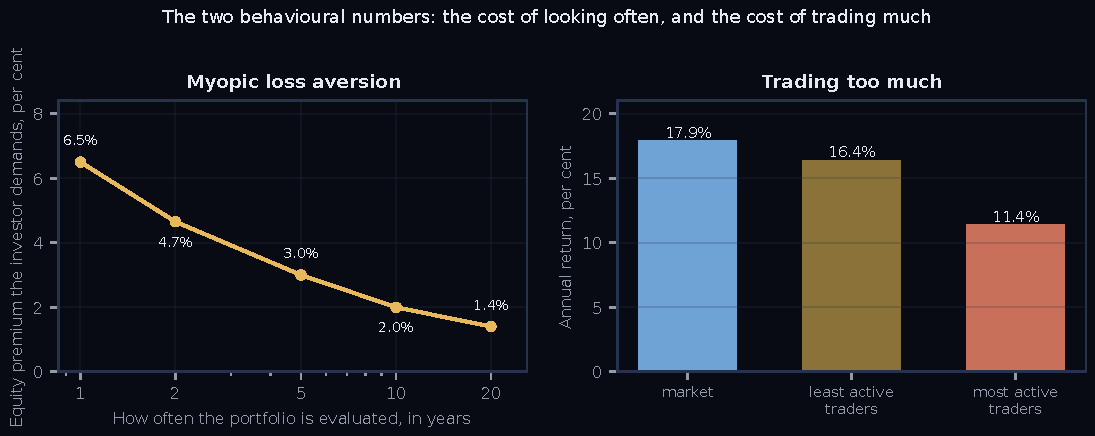
\includegraphics[width=\textwidth]{../figures/fig_behavioural.pdf}
\caption{Three behavioural quantities on a common scale: the loss-aversion
coefficient that drives myopic loss aversion, the excess of realised
returns over what winners sold in the year after a gain (the disposition
effect), and the annual return of the most active retail traders against
the market's.}
\label{fig:behavioural}
\end{figure}

\section{What this implies for a system}

The implication is not that the system should trade less often because
trading is bad. It is that the system should be built so that the investor
has a reason not to interfere with it, and so that the investor's attention
is not drawn to it more often than necessary.

Three concrete design consequences follow, and all three are in the code.

\textbf{The rebalancing frequency is monthly, and it is not the point.}
Monthly is chosen because it matches the data's natural frequency, not
because monthly rebalancing is optimal. What matters is that the
\emph{reported} evaluation frequency of the portfolio is low, and that the
system's own reporting is designed to reduce the number of moments at
which the investor is invited to reconsider.

\textbf{The drawdown brake is designed to prevent re-entry, not to prevent
loss.} A brake that stops the investor from selling during a drawdown
prevents a realised loss but also prevents the recovery. A brake that
pauses new risk and holds the existing allocation through the drawdown
serves the opposite purpose: it reduces the portfolio's exposure at the
moment when the investor is most likely to be looking, and it holds
through the recovery so that the investor who stayed is not punished. The
brake in Chapter 28 does this.

\textbf{Trade only when the trade is worth making.} The system has a
no-trade band. It exists partly to save spread costs and partly for a
behavioural reason: a portfolio that rebalances only when the difference
is material is a portfolio whose statement looks the same most months,
which is a portfolio that is evaluated less often.

\section{The uncomfortable corollary}

There is a reading of this chapter that would make it an argument against
the entire book, and it deserves to be stated rather than avoided.

If the psychic cost of annual evaluation is 5.1 per cent a year, and if a
single investor with one account is structurally more likely to evaluate
annually than an institution with a quarterly reporting cycle and a
committee, then the single investor is the person for whom the behavioural
penalty is largest --- and the machine might be beside the point.

That reading is correct, and the book does not argue against it. What the
book argues is narrower: the machine is worth building if and only if it
makes the portfolio's behaviour automatic, because the alternative --- a
disciplined individual investor following a static policy --- has a much
lower probability of actually doing it. The system's value is not that it
beats the index. Its value is that it is the version of the disciplined
policy that survives contact with the investor's own attention span.

Which is, in the end, the argument for the name of this book.

\begin{keytakeaways}
\item Loss aversion plus a frequent evaluation period raises the premium
the investor believes is required, linearly in the evaluation period; the
premium an investor can actually harvest falls as they look more often.
\item The psychic cost of annual evaluation for a twenty-horizon investor is
5.1 per cent a year --- more than half the historical equity premium.
\item A system built for a single investor must minimise the number of
moments at which the investor is invited to intervene, which is a design
constraint as real as the turnover constraint.
\item The machine's value is that it makes the disciplined policy
automatic; it is not that it beats the index.
\end{keytakeaways}
